\chapter{Механизмы обработки исключительных ситуаций в языке PL/SQL} \label{ch1}

В данной главе рассматривается базовые концепции работы с исключительными ситуациями в языке Oracle PL/SQL.

В параграфе \ref{ch1:sec1} привидена основная информация об ошибках в PL/SQL. В параграфе \ref{ch1:sec2} описаны методы работы с именованными исключениями. Возможности для инициирования исключительных ситуаций описаны в параграфе \ref{ch1:sec3}. Про обработку ошибок рассказывается в параграфе \ref{ch1:sec4}.


\section{Основные концепции обработки исключительных ситуаций в PL/SQL} \label{ch1:sec1}

Исключительными ситуациями в языке PL/SQL считаются любые ситуации, которые не должны возникать при нормальном выполнении программы\cite{ferstein}. 

Под данное определение попадает достаточно большое множество ситуаций, в качестве примера исключений можно привести следующие события: отсутствие данных, ошибки работы экземпляра, непредусмотренные программой действия пользователей. Любая из приведенных выше ситуаций может привести к нежелательному результату, если не будет вовремя найдена и обработана.
 
В языке PL/SQL ошибки перехватываются и обрабатываются в отдельном месте в коде, называемым блок обработки исключений. Такой подход позволяет работать с ошибками как с событиями, передавая управление нужному блоку сразу после возникновения исключительной ситуации, вне зависимости от того в какой конкретно месте возникла данная ошибка. 

Продемонстрируем преимущества такого метода. 
На \firef{fig:c1_code1}, показан вариант линейной обработки ошибок, в таком случае, после каждой команды SELECT мы должны проверить наличие данных.

\begin{figure}[ht!] 
	\center
	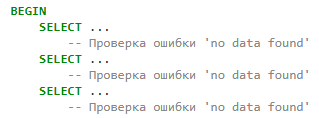
\includegraphics [scale=1] {my_folder/img/C1_code1.png}
	\caption{Пример кода с последовательной обработкой ошибок} 
	\label{fig:c1_code1}  
\end{figure}
\FloatBarrier

Если нам заранее известно, что имеется необходимость во всех данных из каждой команды SELECT, а при отсутствии хотя бы одних из них, мы должны выполнить какие-либо действия, то имеется возможность сильно упростить код, как показано на \firef{fig:c1_code2}.

\begin{figure}[ht!] 
	\center
	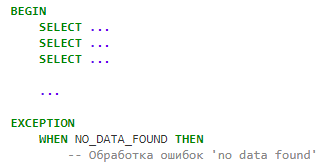
\includegraphics [scale=1] {my_folder/img/C1_code2.png}
	\caption{Пример обработки ошибок в отдельном блоке} 
	\label{fig:c1_code2}  
\end{figure}
\FloatBarrier

В таком случае обработка всех ошибок данного типа будет производиться в одном месте, отлаживать и дорабатывать такую программу будет гораздо проще, по сравнению с первым случаем. 
Также вынесение обработчика в отдельный блок, позволяет отделить логику работы основной программы, от раздела исключений, что позволяет уменьшить количество кода и повысить его читаемость.

В PL/SQL исключения бывают двух типов: системные и пользовательские. Системные исключения – это исключения, которые инициируются ядром PL/SQL в случае нарушением программы правил исполнения установленных Oracle. Пользовательские исключения, в свою очередь, определяются программистом и обычно связаны с конкретным приложением. 

Каждая ошибка имеет свой номер, но обрабатывать исключения можно только по их имени. В Oracle имеется несколько предопределенных ошибок, это часто возникающие ошибки, для которых заданно имя в пакете STANDARD. 

\begin{figure}[ht!] 
	\center
	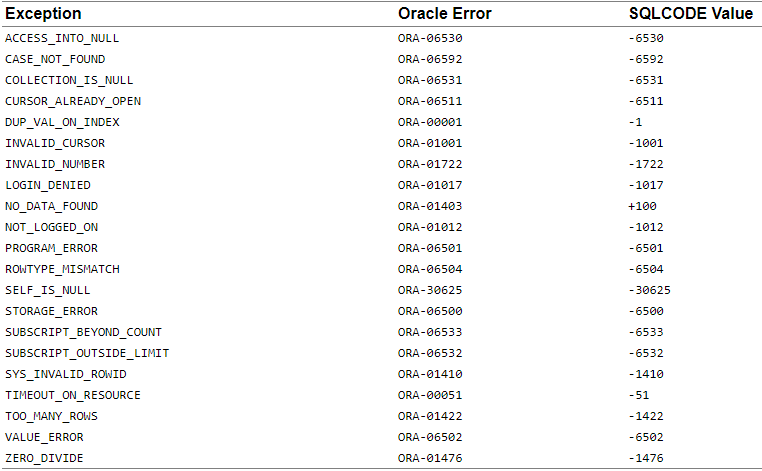
\includegraphics [scale=0.75] {my_folder/img/C1_tab1_predef_exceptions}
	\caption{Предопределенные ошибки из пакета STANDARD} 
	\label{fig:C1_tab1_predef}  
\end{figure}
\FloatBarrier

На \firef{fig:C1_tab1_predef}, приведены примеры предопределенных исключений. 

\section{Определение исключений} \label{ch1:sec2}
В подавляющем большинстве приложений определенных Oracle исключений недостаточно, поэтому необходимо уметь правильно определять и работать с пользовательскими ошибками, которые описывают исключительные ситуации для конкретного приложения.

\subsection{Объявление пользовательских исключений}

Пользовательские исключения позволяют программисту определить новые виды ошибок, для ситуаций, которые не покрываются системными исключениями. 

Очень важной особенностью пользовательских исключений является то, что взаимодейтсвие с ними не отличается от работы с системными ошибками. 

Определение именованных исключений похоже на объявление обычных переменных. Сначала указывается название ошибки, за которым следует ключевое слово EXCEPTION. 

\begin{figure}[ht!] 
	\center
	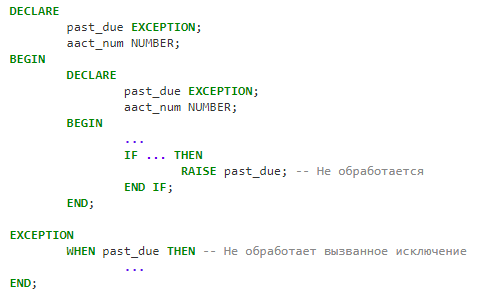
\includegraphics [scale=1] {my_folder/img/C1_exeception_declaration}
	\caption{Пример объявление именованного исключения} 
	\label{fig:C1_exeception_declaration}  
\end{figure}
\FloatBarrier

На \firef{fig:C1_exeception_declaration} показан пример объявления именованного исключения под названием past\_due. Во вложенном блоке объявляется еще одно исключение с таким же именем, так как вложенный блок не имеет обработчика, то его (локальное) исключение past\_due не будет обработано. Внешний блок ничего не знает об исключение past\_due из вложенного блока, поэтому его обработчик не сможет отловить и обработать данное исключение\cite{handling-errors}.

\subsection{Привязка исключений к кодам ошибок}

При помощи директив компилятора можно связать именованное исключение с кодом ошибки. Делается это при помощи команды EXCEPTION\_INIT, в которую передается имя исключения, объявленного ранее, и код ошибки. После такой привязки обращаться к ошибке в разделе WHEN можно по имени. 

Обычно данная директива используется в двух случаях: для задания имени системному исключению, для которого не предусмотренно предопределенного имени, и для работы со специфичными для приложения ошибками.

\begin{figure}[ht!] 
	\center
	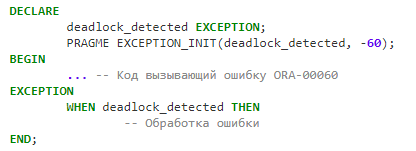
\includegraphics [scale=1] {my_folder/img/C1_exception_init}
	\caption{Пример использования директивы компилятора EXCEPTION\_INIT} 
	\label{fig:C1_exeception_init}  
\end{figure}
\FloatBarrier

В примере показанном на \firef{fig:C1_exeception_init} происходит привязка ошибки с номером -60 к именованному исключению deadlock\_detected.

Хорошим тоном считается вынесение часто используемых ошибок в один пакет и привязка их к номерам, как, например, это сделано в пакете STANDARD со стандартными исключениями. В таком случае, в остальном коде приложения, можно будет обращаться к ошибкам из данного пакета. Следуя такой практике можно повысить читаемость кода за счет стандартизации в определении ошибок.

\section{Инициирование исключительных ситуаций}\label{ch1:sec3}

Существует несколько способов инициировать исключение. В первую очередь, исключения инициируются Oracle в случае возникновения ошибки. Программист может сам инициировать исключения либо при помощи команды RAISE, либо используя процедуру RAISE\_APPLICATION\_ERROR. Рассмотрим последние два способа подробнее.
 
Команда RAISE останавливает нормальное выполнение программы PL/SQL и передает управление обработчику ошибок. Данная инструкция имеет следующий синтаксис.

\begin{figure}[ht!] 
	\center
	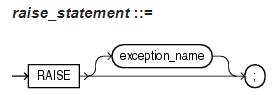
\includegraphics [scale=1] {my_folder/img/C1_raise_syntax}
	\caption{Синтаксис команды RAISE} 
	\label{fig:C1_raise_syntax}  
\end{figure}
\FloatBarrier

Как видно на \firef{fig:C1_raise_syntax} сначала указывается ключевое слово RAISE за которым следует необязательное имя исключения. 

Использование данной команды без указания имени исключения, можно только в разделе WHEN обработчика исключений. В таком случае обрабатываемое в данный момент исключение инициируется повторно, а процесс обработки исключения переходит в родительский блок. Это может быть полезно в случаях, когда нам нужно освободить какие-то ресурсы, либо сохранить какие-либо данные, но что делать с возникшей ошибкой в данный момент времени мы не знаем.

\begin{figure}[ht!] 
	\center
	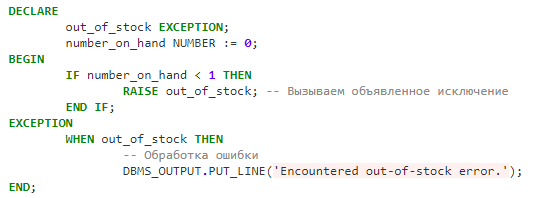
\includegraphics [scale=1] {my_folder/img/C1_raise_example}
	\caption{Пример использования команды RAISE} 
	\label{fig:C1_raise_example}  
\end{figure}
\FloatBarrier

На \firef{fig:C1_raise_example} представлен пример инициирования ошибки с использованием инструкции RAISE. В блоке происходит объявление исключения out\_of\_stock и переменной number\_of\_hand проинициализированной значением 0, после чего в условном блоке происходит проверка значения переменной, если оно меньше 1, то происходит инициирование объявленного ранее исключения, после чего исполнение передается блоку обработки ошибок. 

Другим способом инициировать программисту исключение является процедура RAISE\_APPLICATION\_ERROR из пакета DBMS\_STANDARD.

\begin{figure}[ht!] 
	\center
	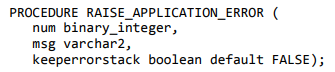
\includegraphics [scale=1] {my_folder/img/C1_raise_application_error_signature}
	\caption{Заголовок процедуры RAISE\_APPLICATION\_ERROR} 
	\label{fig:C1_raise_application_error_signature}  
\end{figure}
\FloatBarrier

Как видно на \firef{fig:C1_raise_application_error_signature} данная процедура может принимать три параметра, два обязательных и один необязательный. Первый параметр – это код ошибки, которую необходимо инициировать, в диапазоне от -20999 до -20000. Второй параметр – это сообщение длиной до 2048 байт, которое будет связано с ошибкой. Третий параметр keeperrorstack указывает, нужно ли добавить ошибку к уже имеющимся в стеке (данное поведение используется при указании значения TRUE), или необходим заменить существующую ошибку (значение FALSE, используемое по умолчанию).

\begin{figure}[ht!] 
	\center
	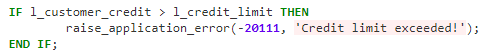
\includegraphics [scale=1] {my_folder/img/C1_raise_application_error_example}
	\caption{Пример использования процедуры RAISE\_APPLICATION\_ERROR} 
	\label{fig:C1_raise_application_error_example}  
\end{figure}
\FloatBarrier

Пример на \firef{fig:C1_raise_application_error_example} демонстрирует использование рассматриваемой процедуры. При нарушении бизнес-логики происходит инициирование ошибки с кодом -20111 с информацией об ошибке. 

\section{Обработка ошибок}\label{ch1:sec4}

При возникновении исключительной ситуации нормальное выполнение PL/SQL кода останавливается, а управление получает раздел обработки исключений, если обработчик данного блока не может справиться с такой ситуацией, то управление переходит в родительский блок. 

Синтаксис блока обработки исключений имеет следующий вид, показанный на рисунке \firef{fig:C1_exeception_handling_syntax}.

\begin{figure}[ht!] 
	\center
	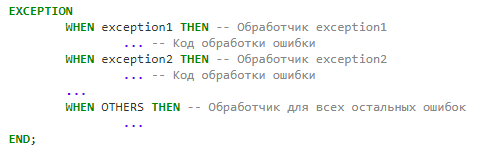
\includegraphics [scale=1] {my_folder/img/C1_exeception_handling_syntax}
	\caption{Синтаксис обработчика ошибок} 
	\label{fig:C1_exeception_handling_syntax}  
\end{figure}
\FloatBarrier

Он может находиться только в конце PL/SQL блока либо вовсе может отсутствовать. Если имя возникшего исключения совпадает с именем, указанным в разделе WHEN, то выполняются команды, находящиеся после ключевого слова THEN. В случае, когда ни один раздел с указанным именем не подходит управление переходит в раздел WHEN OTHERS, если он указан. 

Стоит отметить, что ошибка может быть обработана только одним из разделов. После выполнения команд управление передается в вызывающий блок. 


\section{Получение дополнительной информации об ошибке}\label{ch1:sec5}
Периодически, возникают ситуации, когда необходимо узнать дополнительную информацию об возникшей ошибке. В Oracle не существует возможности расширить объект EXCEPTION и записать туда свою информацию. В базе данных существует несколько функций, которые позволяют получить различную информацию из ошибки. К ним относятся: SQLCODE, SQLERRM, DBMS\_UNTILITY.FORMAT\_ERROR\_BACKTRACE и DBMS\_UNTILITY.FORMAT\_ERROR\_STACK. 
Рассмотрим каждую из них подробнее. 

Функция SQLCODE позволяет получить код возникшей ошибки, если вызвана в блоке обработки исключительных ситуаций, в том случае, если данная функция будет вызвана вне обработчика, то будет возвращено значение 0. Для ошибок, определенных пользователя, возвращается значение +1 или, если функции был присвоен код, при помощи директивы EXCRPTION\_INIT, то данный код и будет возвращен. 
При помощи данной функции можно обрабатывать исключения, которым не присвоены имена, по коду. Пример \firef{fig:C1_handling_by_sqlcode} показывает, как это можно сделать. 

\begin{figure}[ht!] 
	\center
	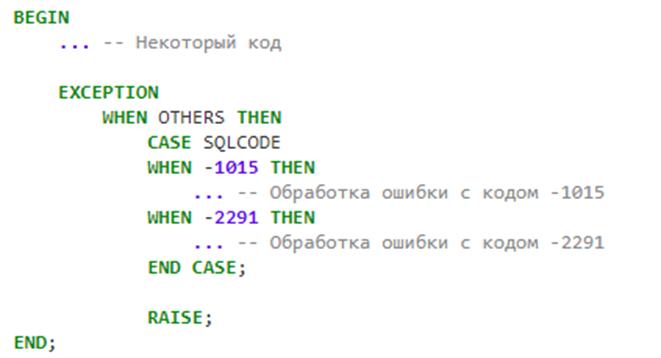
\includegraphics [scale=1] {my_folder/img/C1_handling_by_sqlcode}
	\caption{Обработка ошибок с использованием функции SQLCODE} 
	\label{fig:C1_handling_by_sqlcode}  
\end{figure}
\FloatBarrier

В данном примере, в обработчике ошибок происходит обработка всех ошибок. В случае заданных кодов выполняется особый код только для их обработки, после чего, при помощи команды RAISE снова возбуждается текущее исключение и передается в родительский код. 
Данную задачу можно было бы решить и другим способом, например, связать коды, для которых нужна особая обработка, с именами исключений, и указывать в конструкции WHEN их имена. Такой подход является более предпочтительным, но приведенный пример тоже имеет право на существование.

Функция SQLERRM возвращает сообщение ошибки, связанное с данным кодом. Может принимать в качестве параметра код ошибки. Если вызвана без параметров и в обработчике ошибок, то вернет ассоциированное с текущей ошибкой сообщение. 

Функция FORMAT\_ERROR\_STACK возвращает более подробную информацию об ошибке, в отличии от SQLERRM, помимо сообщения в вывод также включен текущий стектрейс ошибки. Стектрейс - последовательность вызовов и состояние окружения в некоторой точке программы. Преимуществом данной функции относительно SQLERRM является то, что SQLERRM строже ограничен в размерах сообщения. 

Функция FORMAT\_ERROR\_BACKTRACE позволяет получить стек вызова до точки, где была получена ошибка. Эта информация может потребоваться для нахождения причин ошибки. Например, после обработки ошибок, мы записываем в специальную таблицу полученный стек вызова. В дальнейшем, когда, нам будет необходимо исправить эту ошибку, мы можем обратиться к данной таблице и получить всю необходимую информацию о месте ее возникновения. 


\section{Логирование информации об ошибке}\label{ch1:sec6}
Большинство ошибок не может быть исправлено сразу, и не все ошибки требуют моментального исправления. Некоторые будут более приоритетными, некоторые менее, одни ошибки могут возникать очень часто, другие же встречаться крайне редко. Нужно правильно сохранять информацию об ошибках, когда придет время для ее исправления, мы должны иметь возможность получить максимум информации. Oracle предоставляет разработчикам пакет DBMS\_ERRLOG, в котором содержится одна процедура CREATE\_ERROR\_LOG. Данная процедура предназначена для логирования ошибок в DML операциях. 


\begin{figure}[ht!] 
	\center
	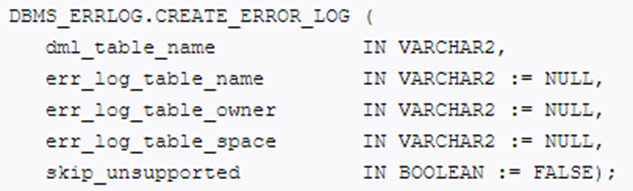
\includegraphics [scale=1] {my_folder/img/C1_create_error_log_syntax}
	\caption{Сигнатура процедуры DBMS\_ERRLOG.CREATE\_ERROR\_LOG} 
	\label{fig:C1_create_error_log_syntax}  
\end{figure}
\FloatBarrier

На рисунке \firef{fig:C1_create_error_log_syntax} представлена сигнатура данной процедуры. Процедура в качестве параметра принимает название таблицы, для которой производилась DML операция, информацию о таблице, в которую нужно занести информацию (таблица логирования) и флаг skip\_unsupported, который позволяет пропустить неподдерживаемые столбцы. К таким столбцам относятся колонки с типами данных LONG, CLOB, BLOB, BFILE и ADT. Если у флага указать значение FALSE, которое стоит по умолчанию, то в случае неподдерживаемого столбца, программа логгирования завершится. 

Данный пакет имеет ряд недостатков. Во-первых, он узконаправленный, сохранение информации об ошибках в не DML операциях, затруднено. Во-вторых, для логирования в нестандартную таблицу, потребуется каждый раз указывать много параметров. В-третьих, мы не можем контролировать информацию, которая будет заносится в таблицу. 

В связи с вышеперечисленным, разработчикам приходится разрабатывать собственный механизм для сохранения информации о возникающих ошибках, специализированный под нужды конкретного кода. 



\section{Выводы} \label{ch1:conclusion}
В ходе данной главы была рассмотрена основная информация об ошибках в PL/SQL. Были изучены инструменты для объявления пользовательских ошибок, для привязки исключительных ситуаций к кодам ошибок, были рассмотрены способы инициирования ошибок и их обработки.

При изучение существующих механизмов обработки ошибок в PL/SQL, были замечены некоторые недостатки и неудобства при работе с ними.  

%% Вспомогательные команды - Additional commands
%
\newpage % принудительное начало с новой страницы, использовать только в конце раздела
%\clearpage % осуществляется пакетом <<placeins>> в пределах секций
%\newpage\leavevmode\thispagestyle{empty}\newpage % 100 % начало новой страницы